\section{Lagrangian formalism}

\subsection{The Lagrangian}    
The Lagrangian $\lagrangian$ is a function that describes the dynamics of a physical system in terms of energy. Mathematically, it is the excess of the kinetic energy of a system over its potential energy, i.e.
\begin{align*}
	\lagrangian(q_i,\dot{q}_i,t)&=T(\dot{q}_i,t)-V(q_i,t),\quad i=1,2,\dots,n \\
	\text{or, }\lagrangian&=T-V
\end{align*}
where the kinetic energy $T$ is a function of generalized velocities and time, and the potential energy $V$ is a function of generalized coordinates and time.

\subsubsection*{Action integral}
Given a system that is described by the Lagrangian $\lagrangian$, its action integral $I$ is defined as the line integral of $\lagrangian$ during the motion of the system from time $t_1$ to time $t_2$, i.e.
\begin{align*}
	I=\int\limits_{t_1}^{t_2}{\lagrangian(q_i,\dot{q}_i,t)\dd{t}}
\end{align*}

\subsection{Hamilton's principle}
\begin{figure}[h!]
	\centering
	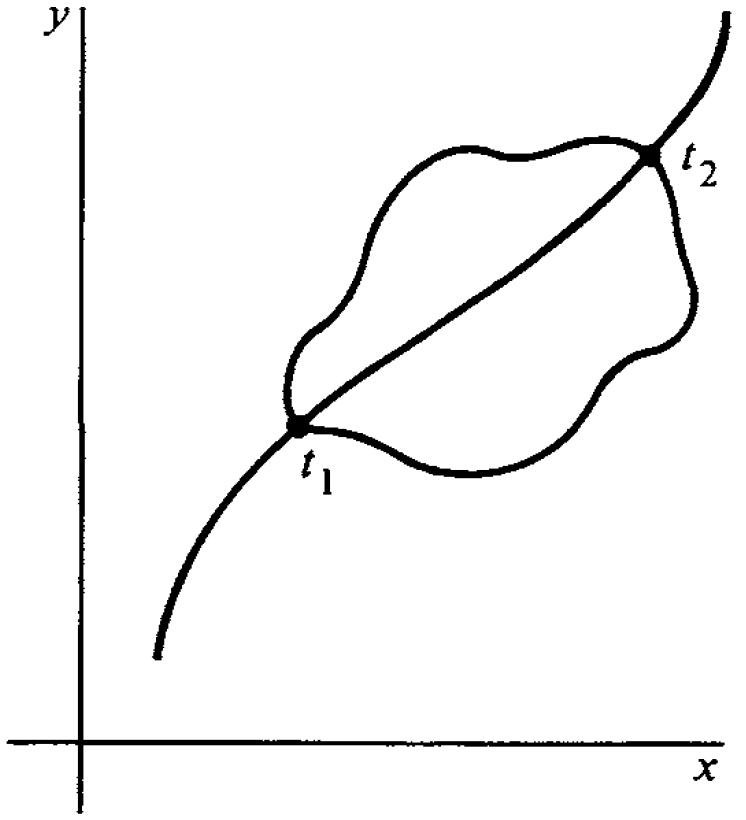
\includegraphics[width=0.4\textwidth]{figures/fig_hamilton-principle.png}
\end{figure}
The motion of the system from time $t_1$ to time $t_2$ is such that the action integral has a stationary value for the actual path of the motion, i.e.
\begin{align*}
	\Aboxed{\delta{I}=\delta\int\limits_{t_1}^{t_2}{\lagrangian(q_i,\dot{q}_i,t)\dd{t}}=0}
\end{align*}
In other words, out of all possible paths by which the system point could travel from its position at time $t_1$ to its position at time $t_2$, it will actually travel along that path for which the value of the action integral is stationary.

\setcounter{equation}{0}
\subsection{Lagrange's equations}
According to D'Alembert's principle, we have
\begin{align}
	\sum_{i=1}^{N}{\qty(\vb{F}_i-\dot{\vb{p}}_i)\cdot\delta{\vb{r}_i}}&=0 \nonumber\\
	\implies\sum_{i=1}^{N}{\vb{F}\cdot\delta{\vb{r}_i}}-\sum_{i=1}^{N}{\dot{\vb{p}}_i\cdot\delta{\vb{r}_i}}&=0 \label{eqn:lag-eqn:dap-terms}
\end{align}
Let us consider the first term in equation (\ref{eqn:lag-eqn:dap-terms}). We have
\begin{align}
	\sum_{i=1}^{N}{\vb{F}\cdot\delta{\vb{r}_i}}&=\sum_{i=1}^{N}{\vb{F}\cdot\sum_{j=1}^{n}{\pdv{\vb{r}_i}{q_j}\delta{q_j}}} \nonumber\\
	&=\sum_{j=1}^{n}{\underbrace{\qty(\sum_{i=1}^{N}{\vb{F}_i\cdot\pdv{\vb{r}_i}{q_j}})}_{=Q_j}\delta{q_j}}\qq{[interchanging summations]} \nonumber\\
	\implies\sum_{i=1}^{N}{\vb{F}\cdot\delta{\vb{r}_i}}&=\sum_{j=1}^{n}{Q_j\delta{q_j}} \label{eqn:lag-eqn:dap-term-1}
\end{align}

Similarly, we now consider the second term in equation (\ref{eqn:lag-eqn:dap-terms}). We now have
\begin{align}
	\sum_{i=1}^{N}{\dot{\vb{p}}_i\cdot\delta{\vb{r}_i}}&=\sum_{i=1}^{N}{\qty(m_i\ddot{\vb{r}}_i)\cdot\qty(\sum_{j=1}^{n}{\pdv{\vb{r}_i}{q_j}\delta{q_j}})} \nonumber\\
	\implies\sum_{i=1}^{N}{\dot{\vb{p}}_i\cdot\delta{\vb{r}_i}}&=\sum_{j=1}^{n}{\qty(\sum_{i=1}^{N}{m_i\ddot{\vb{r}}_i}\cdot\pdv{\vb{r}_i}{q_j})\delta{q_j}} \label{eqn:lag-eqn:dap-term-2a}
\end{align}

Using the product rule for differentiation, we notice that
\begin{align}
	\dv{t}\qty(m_i\dot{\vb{r}}_i\cdot\pdv{\vb{r}_i}{q_j})&=m_i\ddot{\vb{r}}_i\cdot\pdv{\vb{r}_i}{q_j}+m_i\dot{\vb{r}}_i\cdot\dv{t}\pdv{\vb{r}_i}{q_j} \nonumber\\
	&=m_i\ddot{\vb{r}}_i\cdot\pdv{\vb{r}_i}{q_j}+m_i\dot{\vb{r}}_i\cdot\pdv{q_j}\dv{\vb{r}_i}{t} \nonumber\\
	&=m_i\ddot{\vb{r}}_i\cdot\pdv{\vb{r}_i}{q_j}+m_i\dot{\vb{r}}_i\cdot\pdv{\dot{\vb{r}}_i}{q_j} \nonumber\\
	\implies m_i\ddot{\vb{r}}_i\cdot\pdv{\vb{r}_i}{q_j}&=\dv{t}\qty(m_i\vb{v}_i\cdot\pdv{\vb{r}_i}{q_j})-m_i\vb{v}_i\cdot\pdv{\vb{v}_i}{q_j} \nonumber\\
	\implies m_i\ddot{\vb{r}}_i\cdot\pdv{\vb{r}_i}{q_j}&=\dv{t}\qty(m_i\vb{v}_i\cdot\pdv{\vb{v}_i}{\dot{q}_j})-m_i\vb{v}_i\cdot\pdv{\vb{v}_i}{q_j} \label{eqn:lag-eqn:dap-term-2b}
\end{align}
Again, we notice that
\begin{multicols}{2}
	\setlength{\columnseprule}{0.4pt}
	\begin{align*}
		\pdv{q_j}\qty(\dfrac{1}{2}m_iv_i^2)&=\pdv{q_j}\qty(\dfrac{1}{2}m_i\vb{v}_i\cdot\vb{v}_i) \\
		&=\dfrac{1}{2}m_i\times 2\vb{v}_i\cdot\pdv{\vb{v}_i}{q_j} \\
		&=m_i\vb{v}_i\cdot\pdv{\vb{v}_i}{q_j}
	\end{align*}
	
	\columnbreak
	
	\begin{align*}
		\pdv{\dot{q}_j}\qty(\dfrac{1}{2}m_iv_i^2)&=\pdv{\dot{q}_j}\qty(\dfrac{1}{2}m_i\vb{v}_i\cdot\vb{v}_i) \\
		&=\dfrac{1}{2}m_i\times 2\vb{v}_i\cdot\pdv{\vb{v}_i}{\dot{q}_j} \\
		&=m_i\vb{v}_i\cdot\pdv{\vb{v}_i}{\dot{q}_j}
	\end{align*}
	
\end{multicols}
Inserting the above into equation (\ref{eqn:lag-eqn:dap-term-2b}), we obtain
\begin{align}
	m_i\ddot{\vb{r}}_i\cdot\pdv{\vb{r}_i}{q_j}&=\dv{t}\pdv{\dot{q}_j}\qty(\dfrac{1}{2}m_iv_i^2)-\pdv{q_j}\qty(\dfrac{1}{2}m_iv_i^2) \nonumber\\
	\implies\sum_{i=1}^{N}{m_i\ddot{\vb{r}}_i\cdot\pdv{\vb{r}_i}{q_j}}&=\sum_{i=1}^{N}{\qty[\dv{t}\pdv{\dot{q}_j}\qty(\dfrac{1}{2}m_iv_i^2)-\pdv{q_j}\qty(\dfrac{1}{2}m_iv_i^2)]} \nonumber\\
	&=\sum_{i=1}^{N}{\qty[\dv{t}\pdv{T_i}{\dot{q}_j}-\pdv{T_i}{q_j}]} \nonumber\\
	&=\dv{t}\pdv{\dot{q}_j}\sum_{i=1}^{N}{T_i}-\pdv{q_j}\sum_{i=1}^{N}{T_i}\qq{[$T_i$ is K.E. of $i^\text{th}$ particle]} \nonumber\\
	\implies \sum_{i=1}^{N}{m_i\ddot{\vb{r}}_i\cdot\pdv{\vb{r}_i}{q_j}}&=\dv{t}\pdv{T}{\dot{q}_j}-\pdv{T}{q_j} \qq{[$T$ is total energy of the system]} \label{eqn:lag-eqn:dap-term-2c}
\end{align}
Inserting equation (\ref{eqn:lag-eqn:dap-term-2c}) into equation (\ref{eqn:lag-eqn:dap-term-2a}) now gives us
\begin{align}
	\sum_{i=1}^{N}{\dot{\vb{p}}_i\cdot\delta{\vb{r}_i}}&=\sum_{j=1}^{n}{\qty[\dv{t}\pdv{T}{\dot{q}_j}-\pdv{T}{q_j}]\delta{q_j}} \label{eqn:lag-eqn:dap-term-2d}
\end{align}

Finally, inserting equation (\ref{eqn:lag-eqn:dap-term-1}) and (\ref{eqn:lag-eqn:dap-term-2d}) into equation (eqn:lag-eqn:dap-terms), we have
\begin{align*}
	\sum_{j=1}^{n}{Q_j\delta{q_j}}-\sum_{j=1}^{n}{\qty[\dv{t}\pdv{T}{\dot{q}_j}-\pdv{T}{q_j}]\delta{q_j}}&=0 \\
	\implies\sum_{j=1}^{n}{\qty[\dv{t}\pdv{T}{\dot{q}_j}-\pdv{T}{q_j}-Q_j]\delta{q_j}}&=0
\end{align*}
Because, $\delta{q}_j$ is arbitrary, we have
\begin{align}
	\dv{t}\pdv{T}{\dot{q}_j}-\pdv{T}{q_j}-Q_j&=0 \label{eqn:lag-eqn:T-Qj}
\end{align}

Now, if we consider the system to be conservative, we would have $\vb{F}_i=-\vb{\nabla}_iV$ for potential $V=V(q_j)$. Then we have
\begin{align*}
	Q_j&=\sum_{i=1}^{N}{\vb{F}_i\cdot\pdv{\vb{r}_i}{q_j}}=-\sum_{i=1}^{N}{\vb{\nabla}_iV\cdot\pdv{\vb{r}_i}{q_j}}=-\pdv{V}{q_j}
\end{align*}
This gives us, in equation (\ref{eqn:lag-eqn:T-Qj})
\begin{align}
	\dv{t}\pdv{T}{\dot{q}_j}-\pdv{T}{q_j}+\pdv{V}{q_j}&=0 \label{eqn:lag-eqn:T-V}
\end{align}
Because the potential is assumed to be independent of the generalized velocities, we have that $\pdv{V}{\dot{q}_j}=0$ for all $j$. So we can write
\begin{align*}
	\pdv{T}{\dot{q}_j}=\pdv{T}{\dot{q}_j}-\pdv{V}{\dot{q}_j}&=\pdv{(T-V)}{\dot{q}_j} \\
	\implies\dv{t}\pdv{T}{\dot{q}_j}&=\dv{t}\pdv{(T-V)}{\dot{q}_j}
\end{align*}
Therefore, equation (\ref{eqn:lag-eqn:T-V}) becomes
\begin{align}
	\dv{t}\pdv{(T-V)}{\dot{q}_j}-\pdv{(T-V)}{q_j}&=0 \nonumber\\
	\implies\Aboxed{\pdv{\lagrangian}{\dot{q}_j}-\pdv{\lagrangian}{q_j}&=0} \label{eqn:lag-eqn:lagrangeq}
\end{align}
where $\lagrangian=T-V$ is the Lagrangian of the system.

The set of equations given in (\ref{eqn:lag-eqn:lagrangeq}) for each $j$ is known as the Lagrange's equations for a system.